\section{Introducing a data visualization} 
To help people better understand a data visualization design, we propose a method that introduces a data visualization through constructing, which has been proven as an effective teaching method\cite{huron_constructive_2014, chapman_constructive_1988} . Thus, there are three questions we need to answer: ``\textit{what are the basic components that compose a data visualization? }'' ,``\textit{what is the relationship between these components? }'', ``\textit{How should we deal with these relationships in our narrative?}''. At the same time, considering the large number of graphical elements employed in a data visualization design, we should eliminate the visual distraction to keep audience's focus on the target.

\subsection{Compositions of a Visualization}
We propose a model that decomposes a visualization into three levels of structure: visual primitives, visual units, and then an advanced visualization design. 
% We apply this hierarchical structure theory to ``Opinionseer'' and decompose it, as shown in Fig.2. 
We ground our model using OpinionSeer \siwei{[cite]}, a visual design proposed by Wu et al. to \siwei{do sth}. 

\textbf{A visual primitive} is one graphic element \siwei{in the paper, you use graphical element as well. Make them consistent.} whose visual channels, such as color, width, height, are mapped to data attributes. We employ the definition in previous work\cite{huron_constructive_2014, satyanarayan_vega-lite:_2017}, and use the term "grammar" to describe how the visual channels of a visual primitive is influenced by data.\siwei{previous work helps you define visual primitive or grammar? It is not clear} \original{For instance, a point whose size and color are encoded is a visual primitive. How the two visual channels, size and color, are related to data attributes is its visual grammar. }\siwei{I am confused with it. If I understand right, each visual channel is one grammar? In addition, you said you apply the model to OpinionSeer, please refer to the figure and explain what is visual primitive, visual channel and grammar.}

\textbf{A visual unit} is the assembly of visual primitives based on a certain construction rule, as tab.1 show \siwei{please justify how do you define or choose these construction rules?}. 
%For the taxonomy of constructing rule, we refer the ``alignment method'' in \cite{kucher2015text} but make it more specific. 
A visual primitive can assemble different visual units by following different constructing rule, as demonstrated in Fig.3. \siwei{I do not understand this sentence with fig 3. please use an example here.} We are not pretending that our table includes all existing visual units, since new design is proposed constantly. A visual unit is the smallest functional unit of a visualization. Note that people might employ two visual primitives in a visualization design \siwei{what is the relationship between a visualization design and a visual unit? It seems a new term}. For example, \textit{Visual Sedimentation}\cite{huron_visual_2013} \siwei{visual sedimentation has many forms, such as pie chart. Only the bar chart form employs two visual primitives as you describe.} employs two visual primitives, bar and dot, to construct a novel design \siwei{what is the relationship between a design and a visual unit?}. 


\textbf{A visualization} can be treated as the combination of visual units. An naive visualization can be as simple as one visual unit while an advanced one is usually the combination of several units. It doesn't simply put all visual units together but constructs them based on their relationships, as described in Section 3.2.1.
% with certain connections \siwei{what is certain connections? can you give an example?} with each other, which is detailedly discussed in section 3.1.2.\siwei{where is section 3.1.2?}

\begin{figure}
 \centering % avoid the use of \begin{center}...\end{center} and use \centering instead (more compact)
 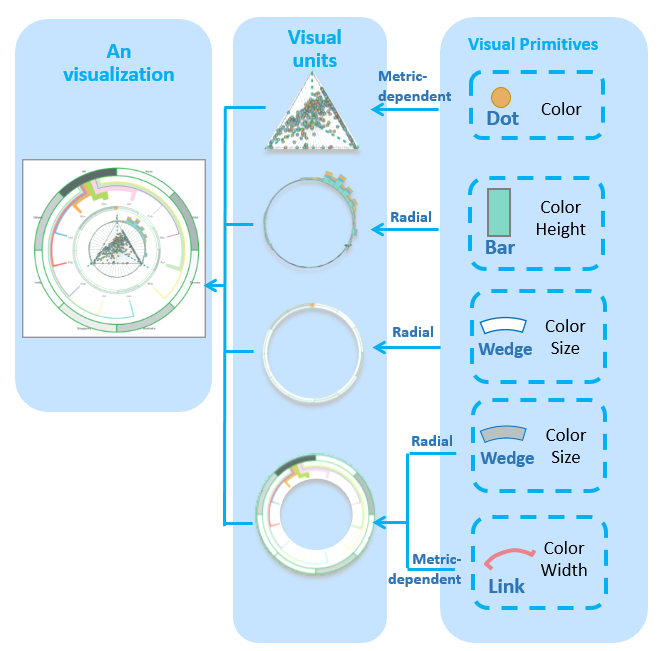
\includegraphics[width=\columnwidth]{hierarchic}
 \caption{An example of the hierarchical structure of a visualization, Opinion Seer\cite{wu_opinionseer:_2010}}
 \label{fig:hierarchic}
\end{figure}

%\begin{figure}
%\begin{minipage}{\columnwidth}
% \centering % avoid the use of \begin{center}...\end{center} and use \centering instead (more compact)
% 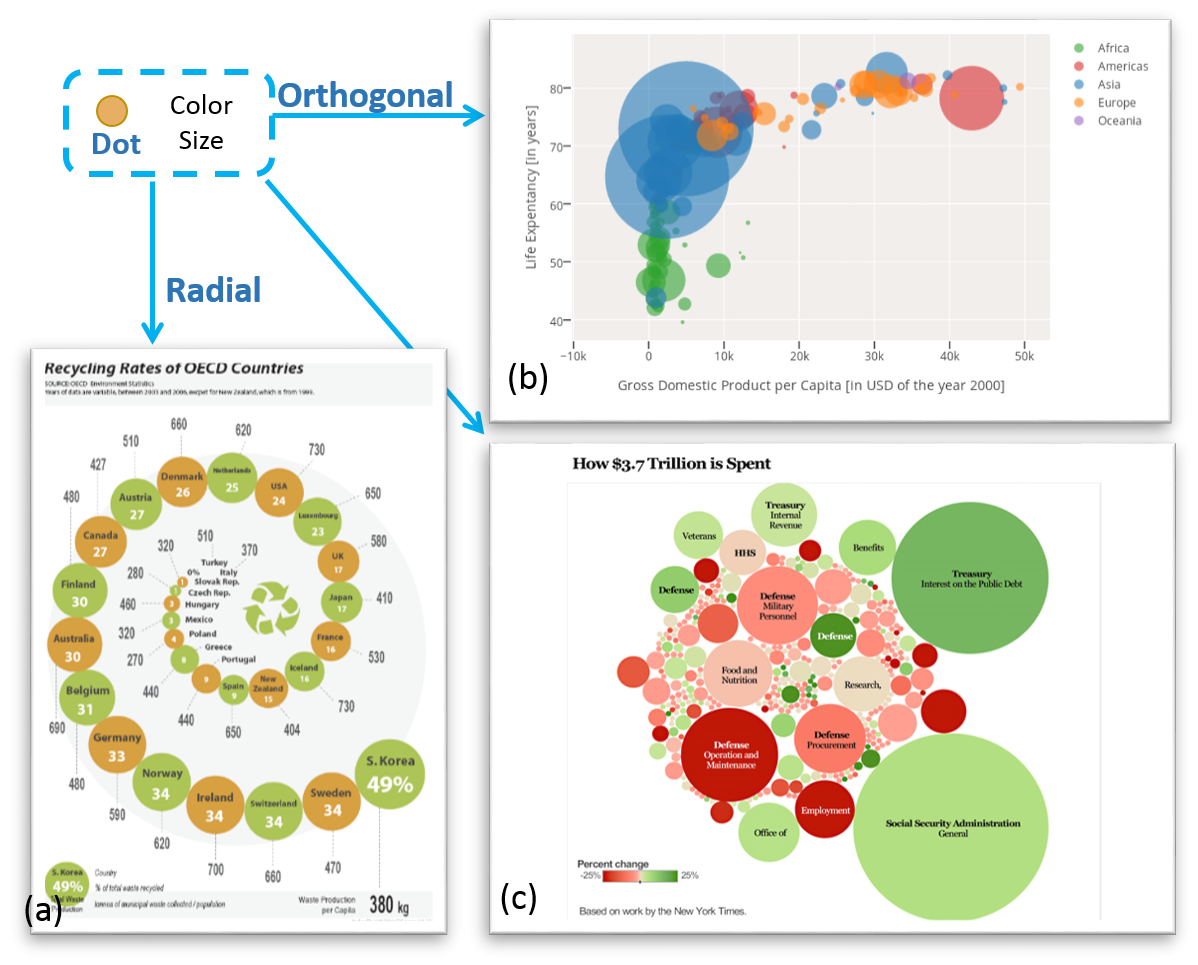
\includegraphics[width=\columnwidth]{assemble}
%\caption[assemble]
%{
%A dot, whose color and size are encoded, can assemble 
%(a) a dot spiral chart
%\protect\footnotemark{}
%    , (b)a dot packing chart
%  \footnotemark{}
%  , and (c)a bubble chart
%  \footnotemark{}
%   by following different construction rules.
%}
%\end{minipage}
%\label{fig:hierarchic}
%\end{figure}
%\footnotetext{https://www.pinterest.com/pin/16536723602037537/}
%\footnotetext{https://plot.ly/~etpinard/84.embed}
%\footnotetext{https://bl.ocks.org/mbostock/4063269}

\begin{table*}[tb]
  \caption{A taxonomy of visual units.\notsure{How to avoid the name ambiguities}}
  \label{tab:unit}
  \small
  \centering
  \begin{tabular}{|p{1.2cm}|p{1.2cm}|p{1.2cm}|p{1.2cm}|p{1.2cm}|p{1.2cm}|p{1.2cm}|p{1.2cm}|p{1.2cm}|}
  \toprule
   \textbf{} &\multicolumn{2}{|c|}{Polar Coordinates} &\multicolumn{3}{|c|}{Orthogonal Coordinates}&\multicolumn{3}{|c|}{Metric Dependent}   \\ 
  \midrule
  
 \textbf{} &\textbf{Radial} &\textbf{Spiral} &\textbf{Orthogonal} & \textbf{Parallel Align}&\textbf{Map}&\textbf{Cluster}&\textbf{Force-direct}&\textbf{Others}   \\ 
  \midrule
  \textbf{Dot} &    &Spiral Dot Chart&Scatter Plot, Bubble Chart & Dot Plot & Bubble Map &  Circle packing    &TopicPanorama\cite{7042494}  &    \\
  \midrule
  \textbf{Line}&  Radar Chart   &  Spiral Plot    &Node-link Diagram, Line Chart & Parallel Coordinates, Arc Diagram &    &   &     & \\ 
  \midrule
   \textbf{Flow}&  Chord Diagram   &    & &Parallel Sets, Sankey Diagram & 
   Flow Map  &   &   &\\
  \midrule
  \textbf{Area}&    &Area Spiral Chart &Stream Graph &  & & &   &\\ 
  \midrule
  \textbf{Bar}&      Radial Bar Chart & Spiral Bar Chart  & Candlestick Chart & Bar Chart  &    &    &    &\\
  \midrule
  \textbf{Cell}& Sunburst Diagram  &    & Matrix, Tree Map &     & & &   &\\
  \midrule
  \textbf{Wedge}& Pie Chart, Donut Chart &  &   &   &  &    &   &\\
  \midrule
  \textbf{Text}&    &Parallel Tag Cloud \cite{collins2009parallel} &    &  Sentence Tree  &     &Word Cloud  &   &    \\
  %\midrule
 % \textbf{Image}& & &Heatmap Matrix &Heatmap &\\
  \bottomrule
  
  \end{tabular}
  \vspace{1mm}
\end{table*}


\subsection{Relationships between compositions}
\subsubsection{Relationships between Visual Units}
% An advanced 
A visualization can be specified as the combination of several visual units. 
% Through observing the approaches people apply to design new visualizations, 
By observing how visualizations are designed,
we define four types of relationship between visual units: irrelevance, relevance, enhancement, and dependency. 

\original{\textbf{Irrelevance} refers to that two visual units have no correlations in the visual grammar. 
It is a bi-directional relation. }
\siwei{combine relationship and narrative seuqence}
\siwei{If I understand right, you can write as: \textbf{Irrelevance} is a bi-directional relation meaning two visual units are independent and do not share any visual channel.}
For example, 2 donut charts, Fig.4(a) and Fig.4(b), are applied to illustrate the distribution of age and gender groups respectively in a population. They are put together in Fig.4(c) just for space-efficiency and there is no correlation between these two charts. \siwei{all figure 4 is figure 3. do not type number. use ref instead}

\textbf{Relevance} refers to that two visual units share some visual grammar and it is a bi-directional relation. 
For example, a line chart, Fig.4(d), and a bar chart, Fig.4(d), share the same encoding of horizontal position and they are put together in Fig.4(e).  \siwei{what is the difference between visual grammar and visual channel? why horizontal position is visual grammar rather than visual channel?}
\notsure{According to our survey, color and position are the most commonly shared visual encodings, which might be the result that color and position usually encoded with simple while crucial information. }

\textbf{Enhancement} is an one-way relationship. If one visual unit ``A'' is the enhancement of another visual unit ``B'', it means that ``A'' is imported into ``B'', replaces some graphical elements of ``B'', thus enables the representation of some data attributes that ``B'' alone fails to convey. Suppose there are 5 types of area in a park. A bar chart, Fig.4(h), illustrates their average price per unit area, a chord diagram, Fig.4(g), illustrates how passengers travel through each area. In Fig.4(i), the bar chart take the place of node segments in a chord diagram, resulting in a novel and informative visualization \siwei{the bar chart and the chord diagram share the same radial position, why not relevance but enhancement? }. 
Some actual examples are the heat map mapped upon the steams in a theme river\cite{wu_opinionflow:_2014}  and usage of glyphs to enhance the meaning of nodes in a multidimensional scaling plot.\cite{chen_peakvizor:_2016}\siwei{if you can explain the `enhancement' clearly with one example, the ``actual example'' seems redundant because you have no figure for them and they are hard to follow.} 

\textbf{Dependence} is an one-way relationship. If one visual unit ``A'' is dependent on ``B'', it means that ``A'' reveal some information that results from the visualization of ``B''. \original{For example, a multiple dimensional scaling (MSD) map, Fig.4(j), shows the similarity between each restaurants in a city. A heat map, Fig.4(h), is then added to the MSD map to show the most common type of restaurants, which information can hardly be obtained from the dataset but quite evident from the MSD map, as in Fig.4(i).}\siwei{I cannot understand the example. First, Fig 3(k) seems contour map rather than heatmap. Second, you cannot say it shows the most common type of restaurants because it depends on your drawing.} The biggest difference between "\textbf{enhancement}" and "\textbf{dependence}" is that \textbf{enhancement} still illustrate the data attributes in the dataset, while \textbf{dependency} reveals the new knowledge we obtain from adopting a previous visualization to the dataset. 

\subsubsection{Relationships Between Visual Primitives}
\siwei{There are some notes: 1. do not mention usually has 1 or 2 primitives. it is flawed. 2. Candlestick chart and error bar are quite similar expect their context. why one has no dependency and the other has logical dependency? 3. do not use two ``such as'' in one sentence.}
The inner relationship between visual primitives is relatively simple.
A visual unit usually has 1 or 2 visual primitives. 

\notsure{
The relationship between the 2 visual primitives, if there are two, are usually self-evident. One primitive either has no dependency on the other one, such as the bar and line in \textit{Candlestick Chart}, or has high and evident dependency.  This dependency can be logical, such as the line and bar in \textit{error bar chart}, or spacial, such as the node segment and arc in \textit{chord diagram}, or temporal, such as the stream and dot in \cite{liu_online_2016}
}

\begin{figure}[tb]
 \centering % avoid the use of \begin{center}...\end{center} and use \centering instead (more compact)
 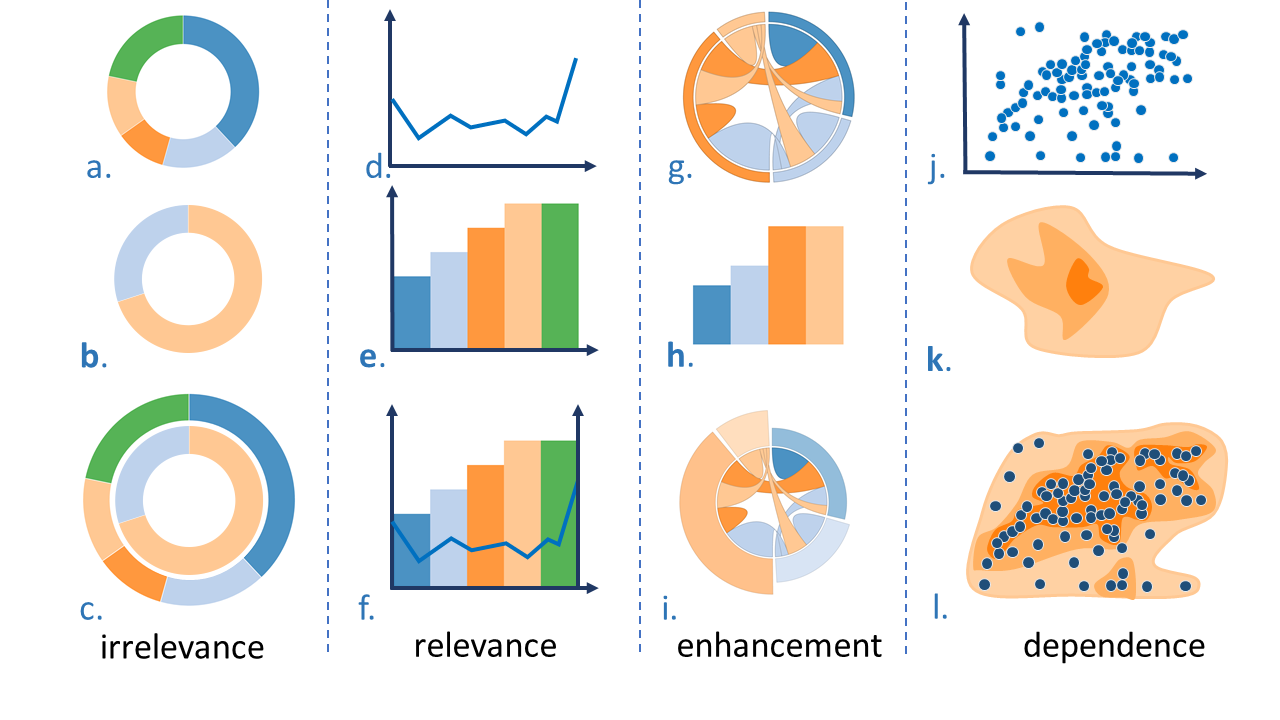
\includegraphics[width=\columnwidth]{unit_relationship}
 \caption{Illustration of the 4 types of relationship between visual units}
 \label{fig:relationship}
\end{figure}

\subsubsection{Relationships Between Visual Channels}
For a visual primitive, different channels are encoded with different data attribute. Thus, they are usually separated and have no logic dependency upon others. 

\subsection{Design considerations of narrative sequence}


\subsubsection{Narrative Sequence for Visual Channels}

\original{An arbitrary explaining order of visual channels may lead to an inefficient information delivery, especially when this visual primitive has multiple channels, which is common in an advanced visualization. }
\siwei{say following an order is important, and why. Do not say arbitrary order is bad. Because other improper order can also be bad.}

Therefore, we define two metrics to order the explaining of visual channels: \textbf{the complexity of their encoded information} and \textbf{saliency of their visual appearance}.

First, a proper explanation should follow the order of decreasing visual saliency~\cite{cleveland_graphical_1984}. Even though different channels have intrinsically different perceptual salience and channel with high salience will suppress the expression of other, such salience strength can be influenced in a task-dependent manner \cite{nothdurft_salience_2000}. By introducing the channel with high saliency first, we remove it from the task list in our mind\cite{itti2001computational}, decrease its saliency and give other channels more chance to attract limited human attention. 

Second, we should follow the order of increasing complexity. “Easy to difficult” practice has been long used and confirmed to be effective for learning new tasks\cite{bliss_effects_1992}.

\siwei{you said we should follow two orders. If they are not the same, which one should I follow?}
 
The visual saliency of different channels is relatively constant and  well defined \cite{munzner_visualization_2014,cleveland_graphical_1984}, while the information complexity varies in different designs. 

\subsubsection{Narrative Sequence for Visual Primitives}
As discussed in section 3.2.2, relationships between visual primitives are self-evident, thus need no special consideration for the narrative sequence. 

\subsubsection{Narrative Sequence for Visual Units} 
As discussed in section 3.1.2, there are four types of relationships between visual units, and they will influence the order of a narrative explanation. Thus, we display the correlations between units in a tree diagram where a child node is the enhancement/dependence of its parent node and sibling nodes have logic dependences. \notsure{as show in Fig}When explaining these visual units, we can simply follow a deep first search (DFS) order to visit all the visual units. \siwei{It is still no clear what is the relationships among: 1) the four relations, 2) the narrative sequence, 3) the tree diagram. For example, how to present irrelevance and relevance using the tree diagram? } 

\subsubsection{Non-linear Sequence}
So far, all the narrative explanation we discussed is linear. However, reading a lengthy, extremely detailed instruction maybe tedious. A good narrative explanation should include non-linear design, allowing users to skip uninterested parts, go back to previous information and freely switch between different parts. Also, users should be allowed the flexibility to choose explanations at different levels of details. 

\subsection{Attention Orientation}
To keep audience focus on the target object, it is necessary for us to identify and avoid visual distractions. 
We identify two kinds of visual distractions: the one from context and the one from sibling channels, which are the visual channels belonging to the same visual primitives. 

\subsubsection{Visual distraction from the context}
This kind of distraction has been widely discussed in the field of object detection and human visual attention \cite{nothdurft_salience_2000, standage_modelling_2005}. Its intensity is mainly  determined by spatial distance and appearance similarity \cite{wolfe_guided_1994}.
\notsure{For example, when we try to focus on a green rectangel, a red triangel near by it can lead to visual distraction. And the intensity of such distraction is determined by the distance and the appearance similarity between the two graphics. Do i need this example} 
Focus + Context, which might be the most popular techniques for this problem, make uneven use of graphic resources to discriminate focus from their context. At the same time, adding dynamic changes to focus elements has also been demonstrated as effective under various conditions\cite{waldner_attractive_2014}. \siwei{it it not clear how the distraction inspires our system? do we take actions to prevent these distraction? do we use focus+context or dynamic changes in our system?} 

\subsubsection{Visual distraction from sibling channels}
A visual primitive usually has more than one visual channels. Thus, when recognizing one primitive, the channels with high visual saliency can significantly influence the expression of other channels. For example, color can be a strong noise when focus is supposed to be the shape. By applying animated transition and revealing only one channel at a time, as demonstrated in \notsure{Fig1, the second line}, we are able to reduce such distraction.


